\documentclass[12pt]{article}\usepackage[english]{babel}\usepackage{emoji}\usepackage{xcolor}\usepackage[hmargin=1in,vmargin=1in]{geometry}\usepackage{amsmath}\usepackage{unicode-math}\usepackage[round,sort,comma]{natbib}\bibliographystyle{apa}\usepackage{setspace}\usepackage{graphicx}\usepackage{caption}\usepackage{subcaption}\usepackage[colorlinks=true, allcolors=blue]{hyperref}\usepackage{float}\usepackage{booktabs}\usepackage{titlesec}\newcommand{\addperiod}[1]{#1.$\;$}\titlespacing{\section}{0pt}{\parskip}{-\parskip}\titleformat{\subsection}[runin]{\normalsize\bfseries}{\thesubsection}{1em}{\addperiod}\titleformat{\subsubsection}[runin]{\normalfont\normalsize\itshape}{\thesubsubsection}{1em}{\addperiod}\titlespacing{\subsubsection}{14pt plus 4pt minus 2pt}{0pt}{0pt plus 2pt minus 2pt}\setlength{\parindent}{1em}\makeatletter\g@addto@macro \normalsize {\setlength\abovedisplayskip{3pt plus 5pt minus 2pt}\setlength\belowdisplayskip{3pt plus 5pt minus 2pt}}\makeatother\newcommand{\comment}[1]{}\begin{document}\pagenumbering{gobble}\begin{center}{\fontsize{16}{16}\selectfont\bfseries \texttt{reproduce.work}: A framework to facilitate cross-platform computational reproducibility in scientific publishing}\\\vspace{5mm}\begin{table}[!ht]\begin{center}\begin{tabular}{c c }\shortstack{ Alex P. Miller \\USC Marshall School of Business \\alex.miller@marshall.usc.edu }\end{tabular}\end{center}\end{table}\vspace{5mm}\emph{Last updated: \today}\vspace{4mm}\hyphenpenalty=10000 \exhyphenpenalty=10000\abstract{In metascience, computational reproduction is the process of reproducing the results of a scientific paper using the data and code provided by the authors of the paper. This subject sits within the broader context of ``reproducibility" in scientific  research, which is the idea that scientific results should be reproducible by other scientists. Concepts around reproducibility have been core to the philosophy of science for decades, but the actual practice of science has fallen woefully short of meeting even basic standards toward true and widespread reproducibility. In this project, we focus primarily on addressing the narrow problem of computational reproucibility. We propose a framework for facilitating computational reproducibility in scientific publishing, which we call reproduce.work. The framework is designed to be cross-platform, and to work with any programming language. It is also designed to be flexible, and to work with any existing workflow. The framework is built on top of the popular nbdev package, which is a tool for developing software in Jupyter notebooks. We showcase the framework by demonstrating the reproducibility of the results of this very paper, which can be run on any machine that can execute a containerized image. We conclude by discussing the potential of the framework for improving rigor and fidelity of computational science for both producers and consumers of published work.
}\\\vspace{2cm}{\scriptsize \noindent Notes: reproduce.work/v0.0.1  \raisebox{-1mm}{
\includegraphics[width=5mm]{../../nbs/img/logo.png}}}\hyphenpenalty=50 \exhyphenpenalty=50\vspace{10mm}\end{center}\newpage\doublespacing\pagenumbering{arabic}\setcounter{page}{1}
\hypertarget{introduction.}{%
\section{Introduction.}\label{introduction.}}

In metascience, computational reproduction is the process of reproducing the results of a scientific paper using the data and code provided by the authors of the paper. This subject sits within the broader context of ``reproducibility'' in scientific  research, which is the idea that scientific results should be reproducible by other scientists (or anyone interested, for that matter). Concepts around reproducibility have been core to the philosophy of science for decades, but several aspects of the scientific method have been challenged by recent developments. 
First, recent conversations around $p$-hacking and fraud in scientific publishing have led to a ``crisis'' at the core of of social science centered around the role of human error, incentives, and guile    . 
Additionally , the increasing computational complexity of scientific research has led to a new set of challenges. Chief among these is the fact that the results of many scientific papers are not reproducible to even the lowest degree. This is because the data and code used to produce the results are not made available to the public.


\hypertarget{background}{%
\section{Background}\label{background}}

advent of computational science has brought new challenges to the field.

At the heart of the concern with research by ousted Stanford president Mark is the fact that it is impossible to verify whether the images produced in the paper are fabricated or actually generated by the scientific equipment they claimed to use in the published manuscript.

The problem of reproducibility is not limited to the field of psychology. 

Reproducibility across the disciplines:
In 2012, the pharmaceutical company Amgen attempted to reproduce the results of 53 landmark cancer studies. They were only able to reproduce the results of 6 of the 53 studies.

In 2015, the journal Science published a study that attempted to reproduce the results of 100 psychology studies. They were only able to reproduce the results of 36 of the 100 studies.

In 2016, the journal Nature published a study that attempted to reproduce the results of 5 landmark cancer studies. They were only able to reproduce the results of 2 of the 5 studies.

In 2018, the journal Science published a study that attempted to reproduce the results of 21 landmark economics studies. They were only able to reproduce the results of 1 of the 21 studies.

this is known as the \href{https://en.wikipedia.org/wiki/Replication_crisis}{replication crisis}.

\hypertarget{related-projects}{%
\subsection{Related projects}\label{related-projects}}

There have been a number of projects with similar aims to this one.

Some work has been done to develop reproducible workflows within specific computing environments. See \href{https://mine-cetinkaya-rundel.github.io/improve-repro-workflow-reproducibilitea-2020/}{example 1} in R.

While some initiatives have emerged to facilitate computational reproduction, there is no widely accepted standard for computational reproduction. 

\hypertarget{an-ontology-of-computation-and-composition}{%
\subsection{An ontology of computation and composition}\label{an-ontology-of-computation-and-composition}}

\begin{figure}[h]
\centering
\caption{Different models of ontology of computation and composition.}
\label{fig:comp}
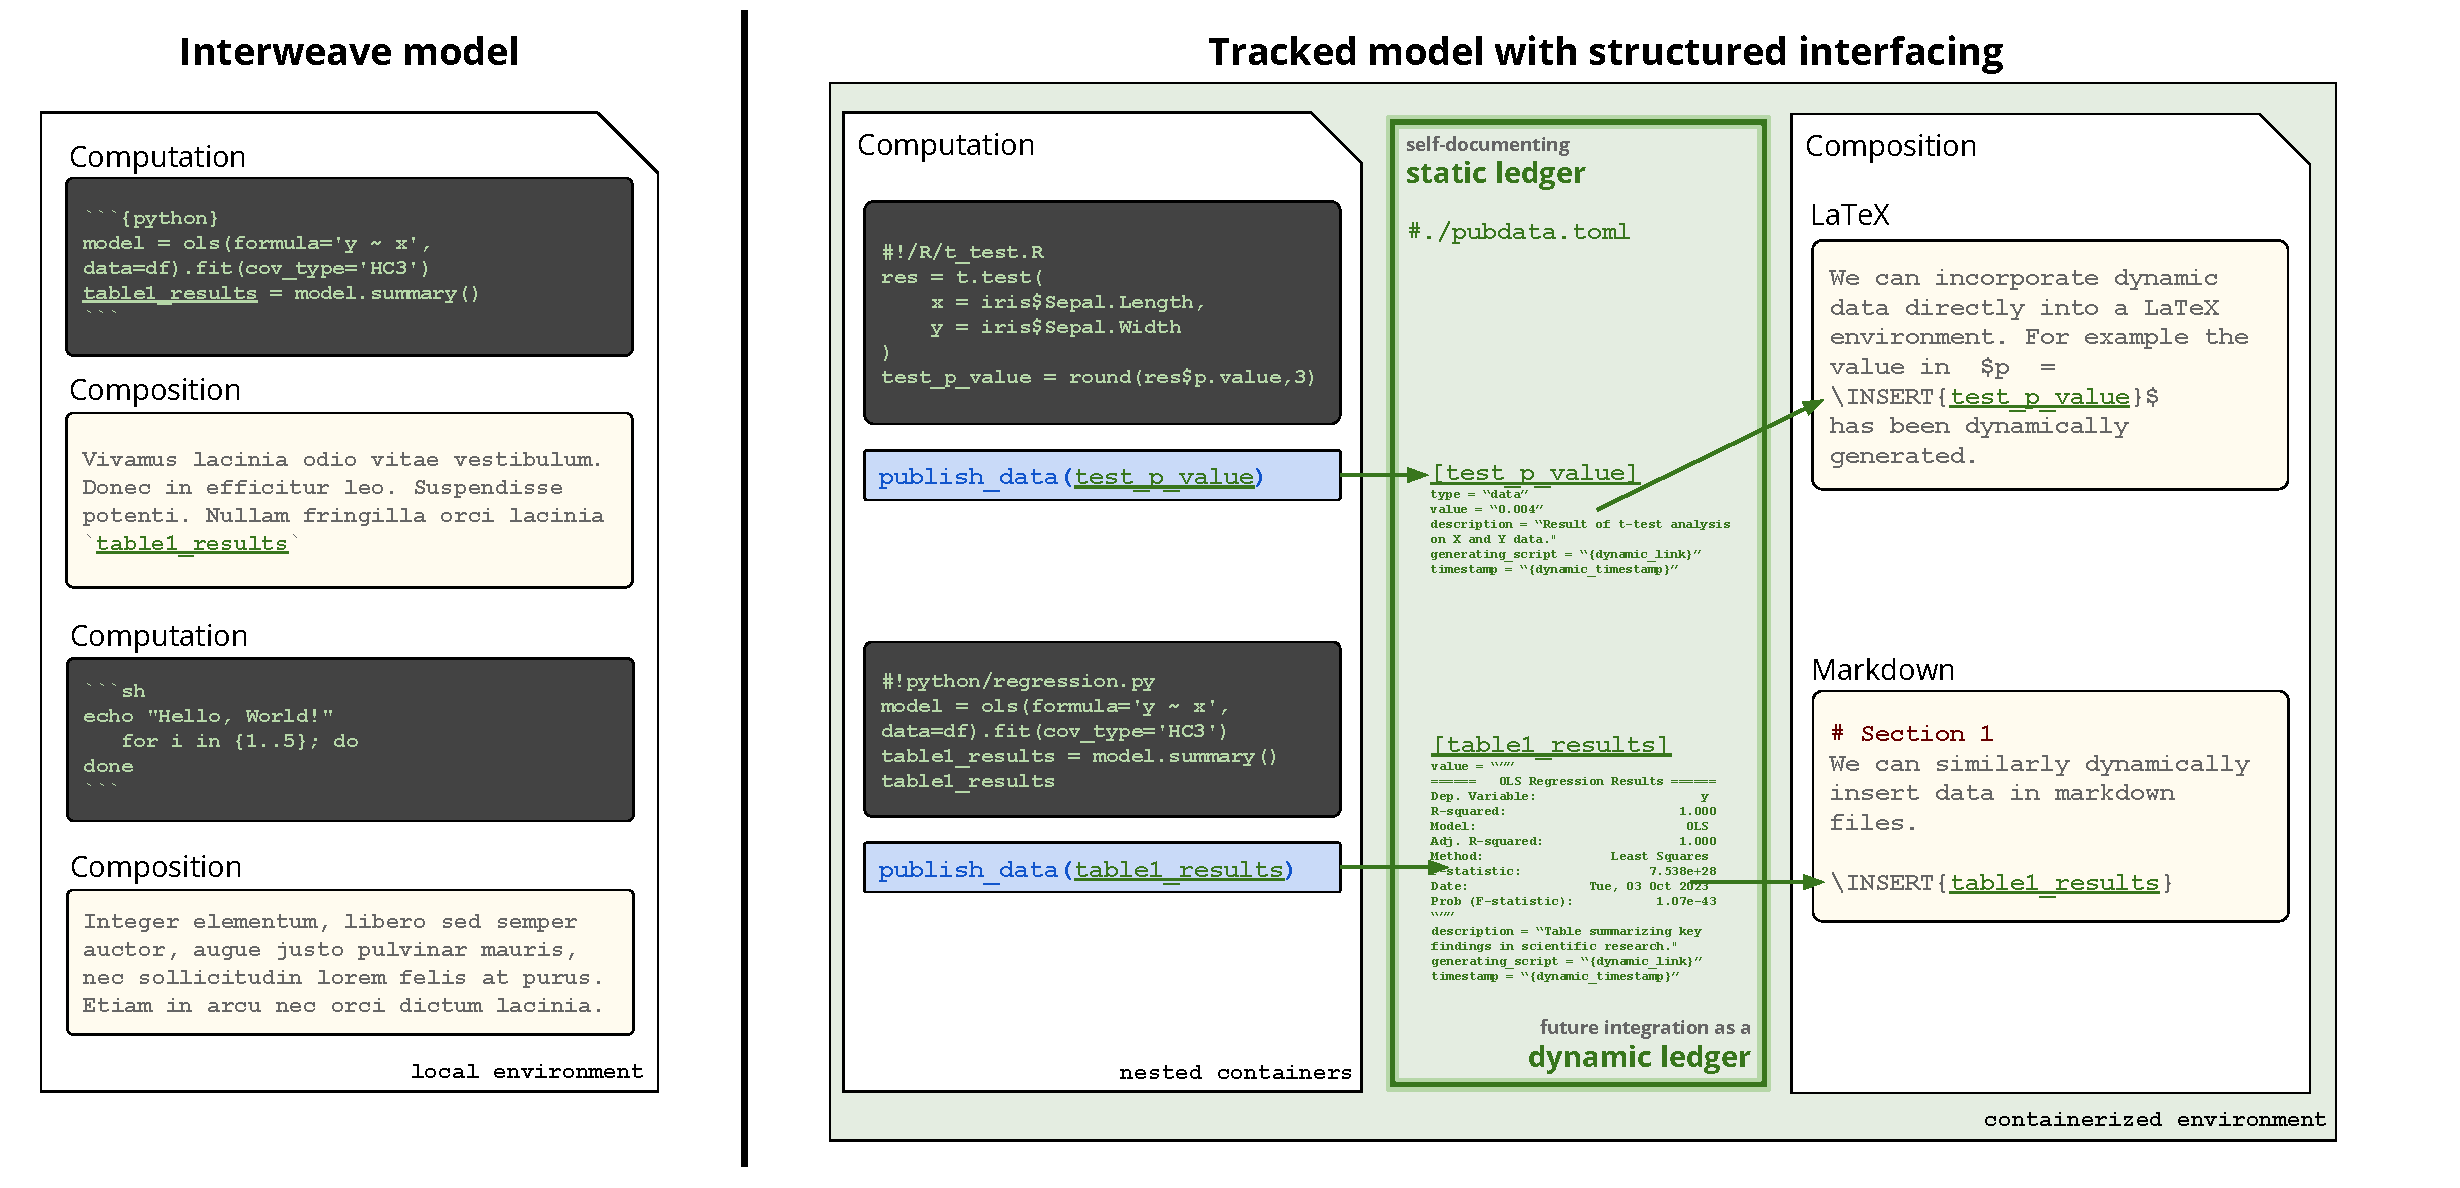
\includegraphics[width=\textwidth]{../../nbs/img/comp.pdf}

\vspace{2mm}
\begin{minipage}{0.95\textwidth}
%\centering
\setstretch{1}
\footnotesize{
\emph{Note:} The \textbf{interweave} model is one in which computation and composition happen linearly within the flow of a single document. Of course, many paradigms including RMarkdown and MyST are quite flexible and allow for a variety of workflows; however, we believe most existing software follows this model. This leads to our proposal of the \textbf{tracked model with structured interfacing}. In this model, the data and code are tracked in a way that allows for easy verification and traceability of reported scientific results with structured metadata.
}
\end{minipage}
\end{figure}

Lay readers may be surprised to learn that the results of many scientific papers are not reproducible to even the lowest degree. (We put forward the following standard as the first of computational reproducibility: ``More than one person verified that the results in the published paper match the results of the code and data provided by the authors.'') 

This is because the data and code used to produce the results are not made available to the public. 

such as the \href{https://rescience.github.io/}{ReScience journal} and \href{https://jupyterbook.org/en/stable/content/myst.html}{MyST Markdown}

While many advocate for the value of peer review in scientific publishing, as of 2023, there no scientific standard exists for true computational reproducibility. 

This is a problem because it means that the quality of peer review varies from journal to journal, and even from paper to paper. 

Do i include \hyperlink{reproduce.work}{0.068}?

the most promising avenue might be emphasizing the importance of collaboration and transparency. By fostering a culture where researchers work together, openly share data and findings, and commit to thorough documentation, the reliability and replicability of work can be increased.

In the coming era, science must not be buoyed by computational power alone, but also by a culture of rigor, collaboration, and transparency.
, the challenge lies not just in advancing science but in ensuring its very foundation remains robust, trustworthy, and verifiable. 

\hypertarget{software}{%
\section{Software}\label{software}}

\hypertarget{seemless-reproducible-scientific-computing-via-containerization}{%
\subsection{Seemless reproducible scientific computing via containerization}\label{seemless-reproducible-scientific-computing-via-containerization}}

Scientific computing is very much like other computing, so it should come as no surprise that tools that have been developed to faciltate the reproduction of arbitrary computing tasks can be adapted to the ends of scientists. Containerization is a technology that allows for the creation of self-contained computing ``containers'' that can be run on any computer with the containerization software installed. While this does necessitate the installation of the containerization software, this is a one-time task that can be done by anyone with a computer. Once the containerization software is installed, the promise of containerization is that a container can be run on any computer, regardless of the operating system or other software installed on the computer. Many containerization standards exist; for present purposes this project uses the \href{https://www.docker.com/}{Docker} containerization standard.

\begin{enumerate}
\itemsep -0.2em
\item inits 
\item build
\item publish
\item verify
\end{enumerate}

\hypertarget{limitations-and-future-directions}{%
\section{Limitations and future directions}\label{limitations-and-future-directions}}

One may ask whether the framework here allows for $p$-hacking type of behavior. To this, we say merely that the framework here is not a panacea; the bar we wished to clear in this first version of the project was to take steps toward a world where computational reproduction is possible. Developing software specifically designed to discourage or encourage certain aspects of human behaviors is a task for future work. 

A key requisite for successful adversarial collaborations is the ability to agree on code and data structure and standards. Being able to easily verify that results correspond to code that was written before but executed after the collection of data.

\hypertarget{conclusion}{%
\section{Conclusion}\label{conclusion}}

In conclusion, this paper has argued that computational reproduction is a promising avenue for improving the quality of scientific research. The project put forward in the body of this project is a mere first step in the direction of computational reproduction. The software lacks support for many important features and the concept is heretofore untested. However, given the low bars required to improve the existing practices around computational reproduction, we beleive this project and the ideas put forward here have potential as the seed of a revolution in reproducibility.
\bibliography{latex/bibliography}\end{document}